\section{Methods}

To archive clustering, the method adopted was to compare document using the authorship linkings strategies presented in \cite{kocher_verification}.
In \cite{kocher_verification} the authors compared multiple text representation based on author style : words frequencies, lemma frequencies, Part-Of-Speach (POS) tags frequencies, short sequences of POS tags, as well as n-grams frequencies.
The distance mesures used are : $L^1$ norms (Manhattan, Tanimoto), $L^2$ norm (Matusita, Clark), inner products (Cosine distance) and the Jeffery divergence.
Depending on the dataset, the text representation and the metric used, no clear text representation and different distance mesures were giving better or worse results.

In this study to archive a good clustering, the main objective is to have a reliable authorship linking rank list.
To try to increase the quality of the rank list, the proposed method is to use a combination of multiple rank list using different strategies to form a hopefully better rank list.
By using the most diverse strategies, we belive it is possible to increase the quality using the principle of combinaison of evidences.

\subsection{Authorship linking}

The next sections will present, different stylistic text representations to create the authorship linking rank list. They are mostly based on the text representation proposed in \cite{kocher_verification}.

\subsubsection{Word Tokens}

The first method is rather simple but yet effective where we consider each token as a word.
In the datasets used, the tokenization is already done such that each word is correctly tokenized.

\subsubsection{Letters n-grams}

For this method, instead of considering every token as a word, we create word from short sequences of letters called n-grams using Definition~\ref{def:n-grams}.
To consider overlapping word, the whole document is synthetized to a long string by joining every token by a \textit{underscore} : $\_$.

\begin{definition}[$N$-Grams]
  \label{def:n-grams}
  A $N$-gram is a special type of tokenization which is constructed by creating a token for the substrings from $0$ to \textit{text\_size} - $N$ of size $N$.
  Example: Using 3-grams The string: "brown fox" is converted to: \\
  $("\text{bro}", "\text{row}", "\text{own}", "\text{wn\_}", "\text{n\_f}", "\text{\_fo}", "\text{fox}")$
\end{definition}


\subsubsection{POS n-grams}

To detect another stylistic aspect of a text, this method aim to consider the sentence constructions of the authors using short sequences (n-grams) of POS tags.

For example, the sentence : \textit{"The cat eat a fish"} has the following POS tag \textit{"Article Noun Verb Article Noun"} which correspond to the following 3-gram of POS : \textit{"Article Noun Verb"} / \textit{"Noun Verb Article"} / \textit{"Verb Article Noun"}.
In practice the POS is more detailed, for example instead of just considering the verb, the verb and it's tense can be used, same for the other type of POS.

Figure~\ref{fig:pos_ngrams} show the average precision on the rank list produced by using POS n-grams over the number of MFW (most frequent word, in this case POS n-grams are considered as words).
The two following informations can be intuitively observed on this plot:

A more complex POS n-gram requirement more MFW to archive its maximal effectiveness.
In the St-Jean corpus 26 POS are used to describe every words in the corpus.
Which correspond to $26^2 = 676$ possible unique POS 2-grams, to $26^3 = 17'576$ POS 3-grams and $26^4 = 456'976$.

Like the other methods, an overfit to less important words is possible if the MFW ceiling is too high, reducing the average precision.
In Figure~\ref{fig:pos_ngrams} the POS 2-grams clearly have drop in average precision after \~250-MFW.

\begin{figure}
  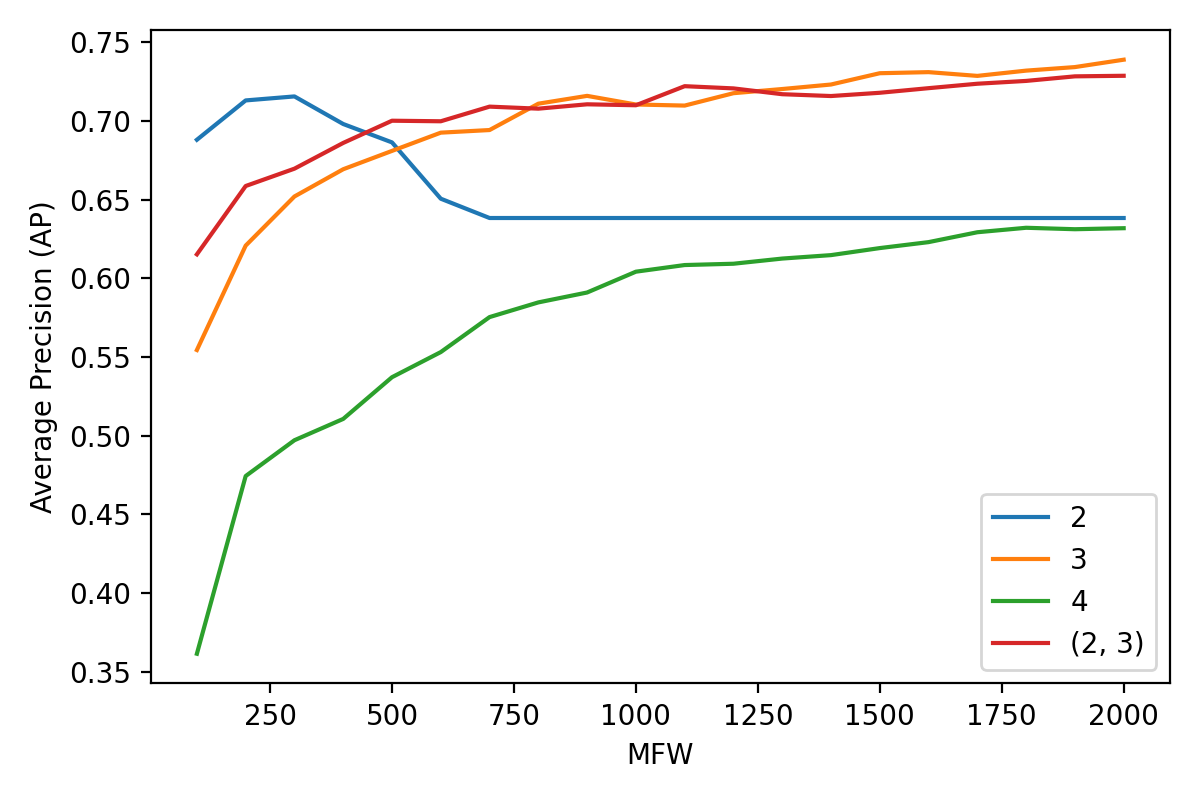
\includegraphics[width=\linewidth]{img/pos_ngrams.png}
  \caption{Average precision over the MFW in the rank list generated using the z-score normalized cosine distance.}
  \label{fig:pos_ngrams}
\end{figure}

\subsubsection{First letters, last letters of tokens}

With this methods, the goal is to extract the N first letter of each word tokens which correspond generaly to the meaning of a word.
This approach is closely related to the lemma approach.
Extract also the N last letter of each word tokens which in this case correspond to the role of the word in a sentence.
This second approach is closely related to the POS approach.

These two methods can be considered as simplified n-grams approach of the same size.

Figure~\ref{fig:first_last_letters_ngrams} shows the average precision using the z-normalized cosine distance on the experiment for N = 4.

\begin{figure}
  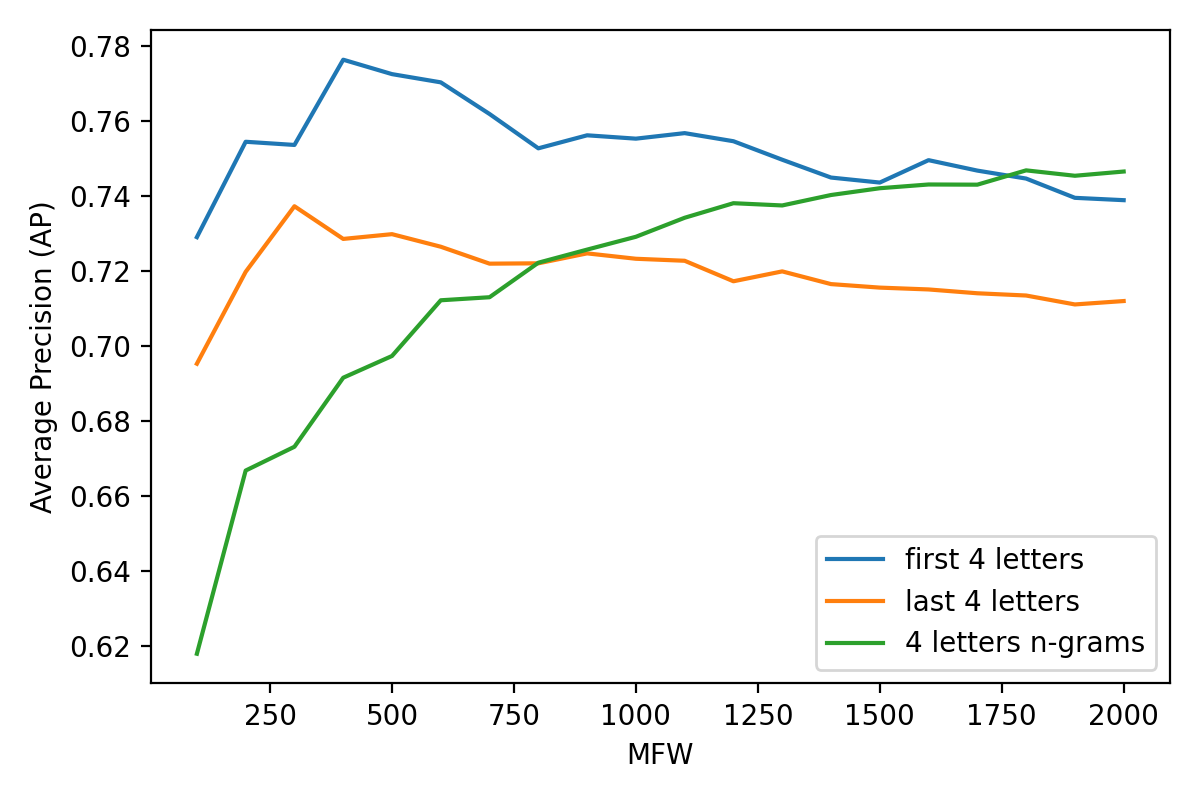
\includegraphics[width=\linewidth]{img/first_last_letters_ngrams.png}
  \caption{Average precision over the MFW in the rank list generated using the z-score normalized cosine distance.}
  \label{fig:first_last_letters_ngrams}
\end{figure}


\subsubsection{Frequent errors}

This section, try to understand the errors in our system, in this case the false links (document pairs with different authors) highly ranked on different rank list.
The rank list quality is highly based on the feature vector created using the N-MFW, having a good understanding of this vector give good indications of the strength of the system.

To find reccurant errors in our system we use 5 different distance metrics on the relative frequency of the 500-MFW using the St-Jean dataset.
This generate 5 rank lists.
The average precision for these rank list is always greater than 0.7.
With this 5 rank lists only the top 10 false links are kept to be analyzed.
Frequent errors are link that appear often in this top 10.
Figures~\ref{fig:mfw_vector_error_0}~/~\ref{fig:mfw_vector_error_1} show two pairs (Zola 49 / Flaubert 63 and Maupassant 10 / Flaubert 52) that appear 4 time out of the 5 rank lists in the top 10 false links, thus frequent error.

\begin{figure}
  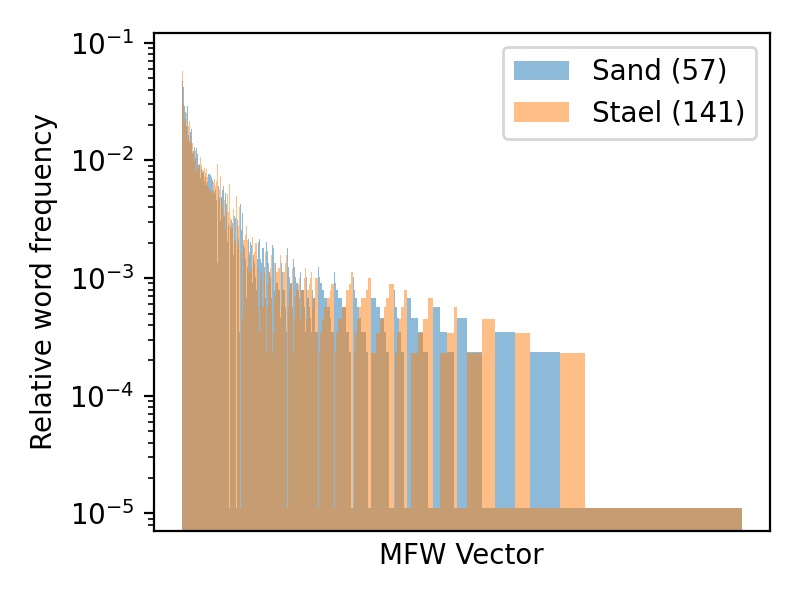
\includegraphics[width=\linewidth]{img/mfw_vector_error_0.png}
  \caption{First example of 500-MFW relative frequency vector for the two documents in a reccurant (4 rank lists out of 5) false link in the top 10 false links}
  \label{fig:mfw_vector_error_0}
\end{figure}
\begin{figure}
  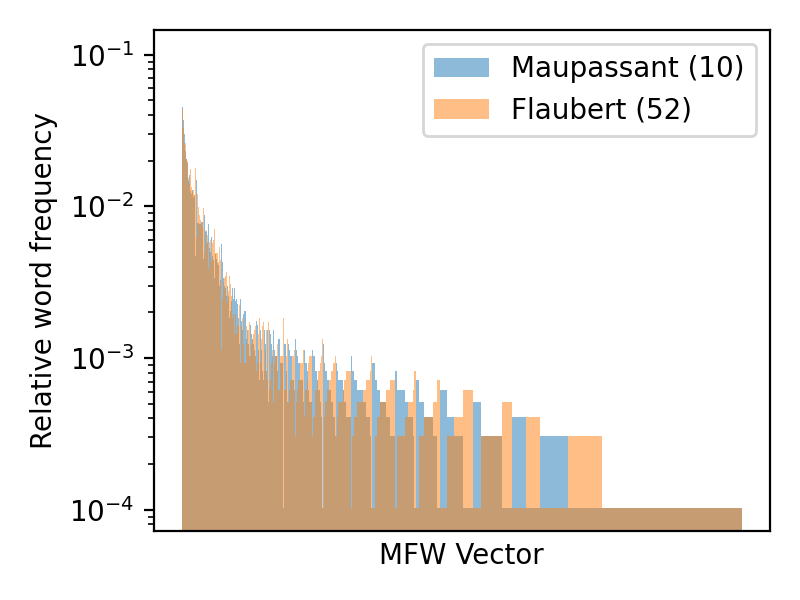
\includegraphics[width=\linewidth]{img/mfw_vector_error_1.png}
  \caption{Second example of 500-MFW relative frequency vector for the two documents in a reccurant (4 rank lists out of 5) false link in the top 10 false links}
  \label{fig:mfw_vector_error_1}
\end{figure}

To be able to understand more easily this vector, the values have been sorted by relative frequencies.
When a large propostion of the vectors overlap it indicates a high similarities between the vectors.
In this case most of the surface overlap so the distance function will give a low value, and rank this vector high in the list.
Both document style are close when their feature vector are closely related.
We can't clearly determinate that these texts are from different author using only this type of representation.
These two vectors pair can be vizually compared to the most similar link (ranked 1 using manhattan distance) in Figure~\ref{fig:mfw_vector_first_rl} (Stael 157 / Steal 183) or the HPrec-th (last continous correct pair from the top of the list) in Figure~\ref{fig:mfw_vector_first_last_rl} (Maupassant 10 / Maupassant 67), both of these links show a large propotion of overlapping surface.
A counter example would be the least similar link (ranked last using manhattan distance) which represent a negatively correlated document pair, Figure~\ref{fig:mfw_vector_last_rl} showcase this link.
As expected, most of this figure surface is non-overlapping.

\begin{figure}
  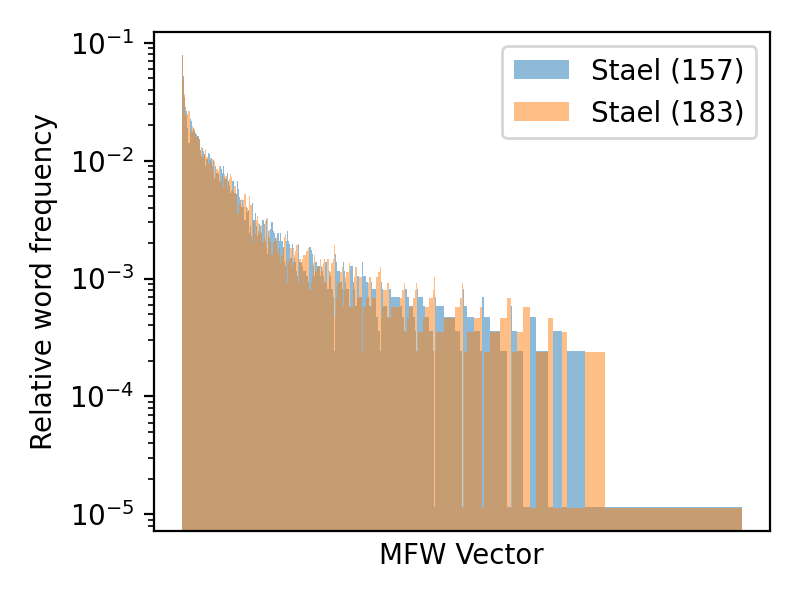
\includegraphics[width=\linewidth]{img/mfw_vector_first_rl.png}
  \caption{500-MFW relative frequency for the two documents ranked first in the rank list}
  \label{fig:mfw_vector_first_rl}
\end{figure}
\begin{figure}
  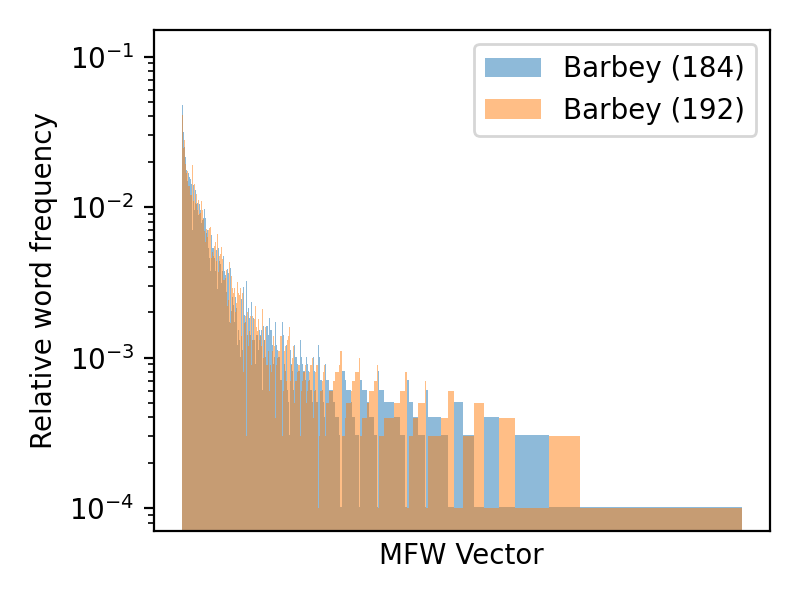
\includegraphics[width=\linewidth]{img/mfw_vector_first_last_rl.png}
  \caption{500-MFW relative frequency for the two documents ranked HPrec-th in the rank list}
  \label{fig:mfw_vector_first_last_rl}
\end{figure}
\begin{figure}
  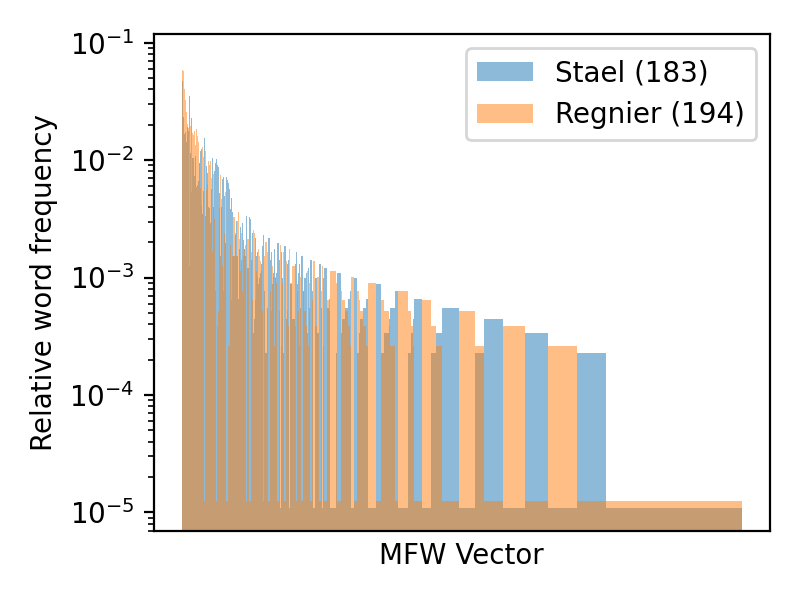
\includegraphics[width=\linewidth]{img/mfw_vector_last_rl.png}
  \caption{500-MFW relative frequency for the two documents ranked last in the ranked list}
  \label{fig:mfw_vector_last_rl}
\end{figure}

\subsubsection{Publication date differences analyis}

When dealing with false links ranked high in the rank list, as the previous experiment showed, some excerpt use similar words.
These shared words might be related to era the book was written.
The following experiment try to investigate on this.

First we must understand the publication date distribution of dataset. Figure~\ref{fig:dates_distribution} show this distribution.
Figure~\ref{fig:dates_differences_all} show the date difference distribution for each pairs of document, we can see that the average date difference in the dataset is 28.24 years with a standard deviation of 20.73 years.
Since this dataset contain multiple excerpt from the same book, we might consider only the links of differents authors (false links) Figure~\ref{fig:dates_differences_false} show such distribution.
As expected the mean increased to 29.04 years since there are less links with small date difference.
Same authors links (true links) are displayed in Figure~\ref{fig:dates_differences_r_true}, they confirm the previous statement that most of the same authors links have a low date difference with a mean at 5.11 years.

\begin{figure}
  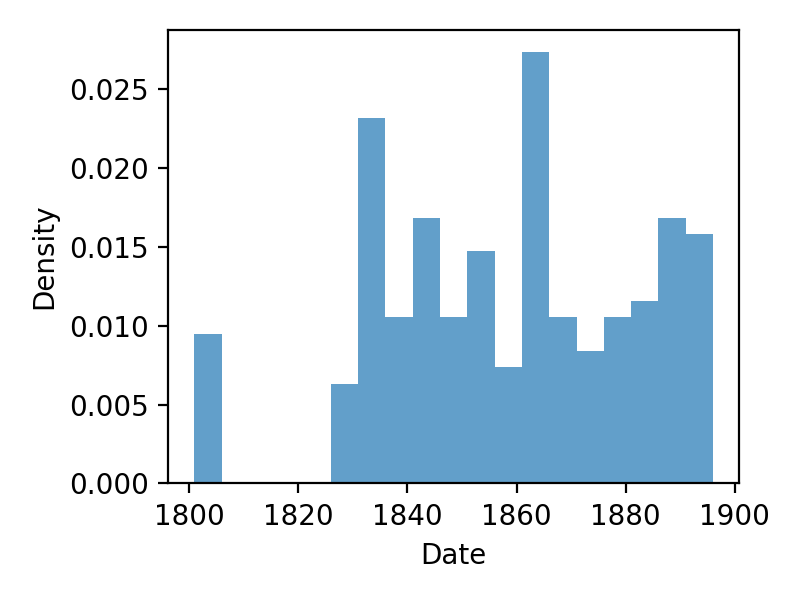
\includegraphics[width=\linewidth]{img/dates_distribution.png}
  \caption{Date distribution in the St-Jean dataset.}
  \label{fig:dates_distribution}
\end{figure}
\begin{figure}
  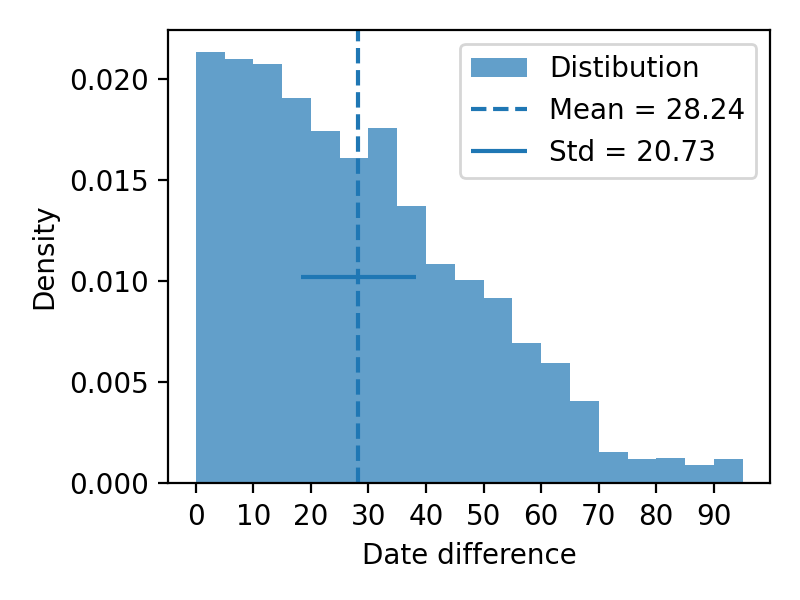
\includegraphics[width=\linewidth]{img/dates_differences_all.png}
  \caption{Pairwise date difference denstiy in St-Jean for all the excerpt.}
  \label{fig:dates_differences_all}
\end{figure}
\begin{figure}
  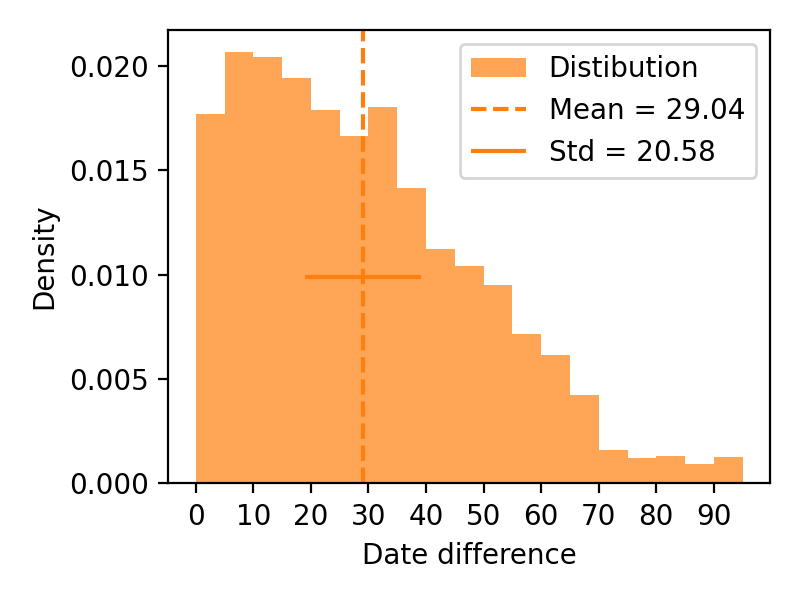
\includegraphics[width=\linewidth]{img/dates_differences_false.png}
  \caption{Pairwise date difference denstiy in St-Jean for all the excerpt with different authors (false links).}
  \label{fig:dates_differences_false}
\end{figure}
\begin{figure}
  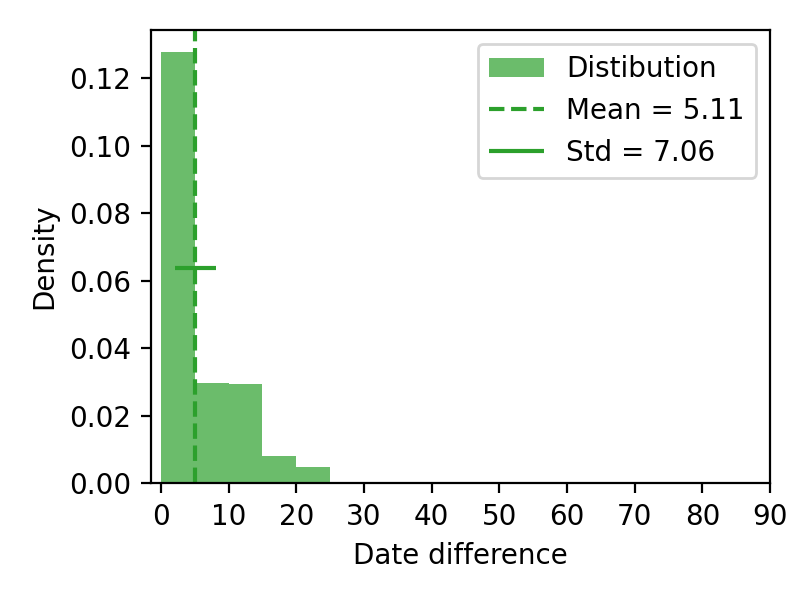
\includegraphics[width=\linewidth]{img/dates_differences_r_true.png}
  \caption{Pairwise date difference denstiy in St-Jean for all the excerpt with similar authors (true links) also correspond to the top-r true links.}
  \label{fig:dates_differences_r_true}
\end{figure}

Figure~\ref{fig:dates_differences_r_false} show the date difference density on the top-r false links (670 in case of St-Jean) on a rank list with 80\% average precision.
Two interesting informations can be extracted here.
First the mean is lower by 8.22 years (29.04 - 20.82) comparing to the false links distribution which clearly indicate a importance of publication date in the ranking of the documents.
Secondly we can obseve a drop at 35 years of date difference, which indicate that links in the interval $\left[0-35\right]$ are harder to discriminate than links outside this interval.
This 35 years interval can be related to the generation factor, the age of woman giving birth is around 25-34 in France \cite{generations}.
Each new generation use its own vocabulary and can be harder to discriminate author of text beloning to the same generation, in the other hand having differant vocabulary can indicate a differant time periode and is often use to detect document forgery \cite{savoy_stylo}.

\begin{figure}
  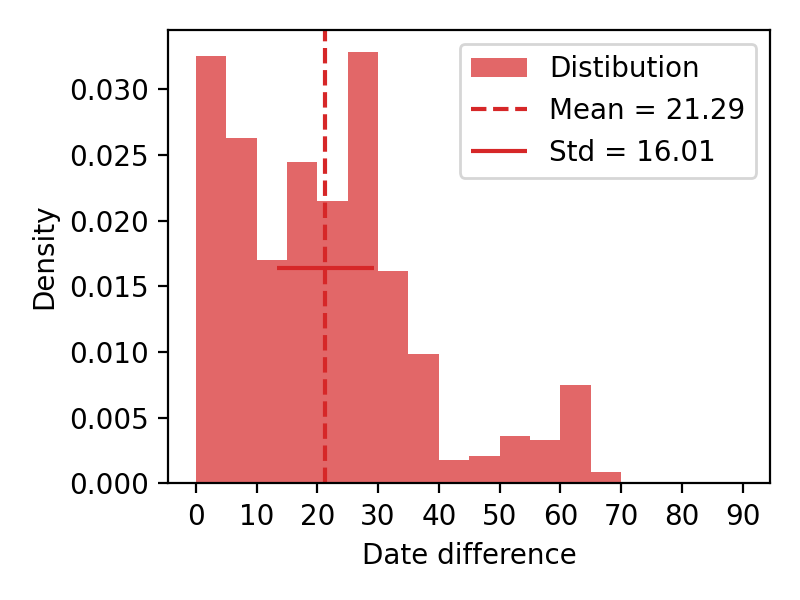
\includegraphics[width=\linewidth]{img/dates_differences_r_false.png}
  \caption{Pairwise date difference denstiy in St-Jean for top-r false links using a rank list with 80\% average precision.}
  \label{fig:dates_differences_r_false}
\end{figure}

\subsubsection{Rank list fusion}

Each rank list is ordered by a score, this score depend on distance measure used, thus the order of magnitude of each rank list is different.
To avoid having to problems in merging rank list with different magnitude, the solution opted is to only use the rank of each link.

An additional constraint desired is to favor top ranked link and penalize bottom ranked links when fusing rank lists.
This constraint can be easily explained by observing the distance over the rank graph of the rank list.
Figure~\ref{fig:distance_over_rank} clearly show us the top ranked links and bottom ranked links have a more sharper decision than in than the middle section.

\begin{figure}
  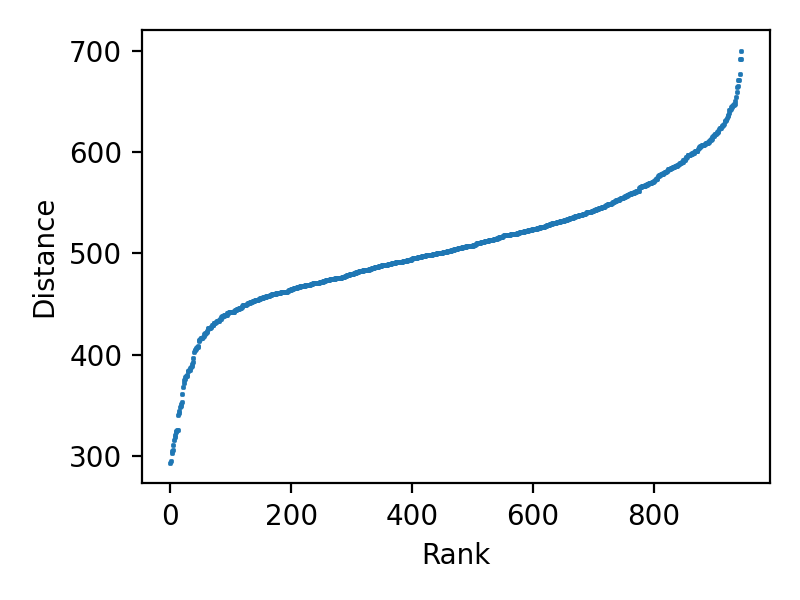
\includegraphics[width=\linewidth]{img/distance_over_rank.png}
  \caption{Distance over rank in the links of the Brunet dataset using Manhattan distances using the 500 most frequent tokens.}
  \label{fig:distance_over_rank}
\end{figure}

Top ranked links correspond to similar documents and bottom links correspond to negatively correlated documents.
Assuming that the top rank are true links after the rank list fusion these link should also be top rank.
The same reasoning can be apply for the bottom links by assuming them as false links.
A weighting curve must be design accordingly.
Using the reciprocal of the sigmoid function we can modelize such curve.
Sigmoid functions presented in Equation~\ref{eq:sigmoid} and Figure~\ref{fig:sigmoid}.
It's reciprocal in Equation~\ref{eq:sigmoid_r} and Figure~\ref{fig:sigmoid_r}.

\begin{equation}
  \label{eq:sigmoid}
  S(x) = \frac{1}{1+e^-x}
\end{equation}
\begin{equation}
  \label{eq:sigmoid_r}
  S^{-1}(x) = -\ln{\frac{x-1}{x}}
\end{equation}

\begin{figure}
  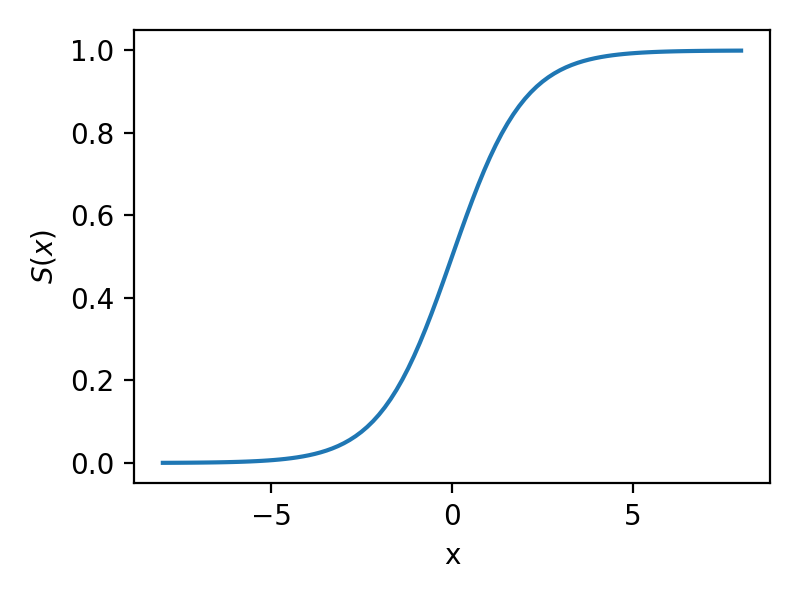
\includegraphics[width=\linewidth]{img/sigmoid.png}
  \caption{Sigmoid function between -4 and 4}
  \label{fig:sigmoid}
\end{figure}
\begin{figure}
  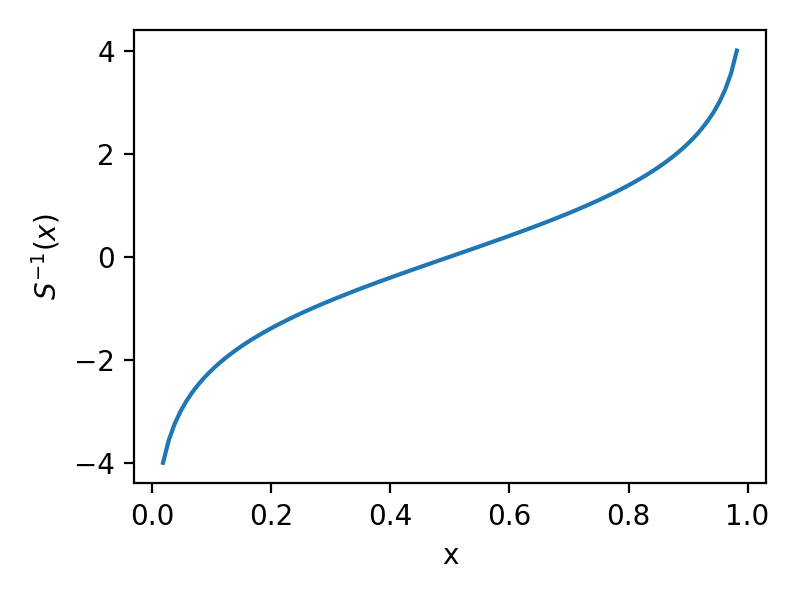
\includegraphics[width=\linewidth]{img/sigmoid_r.png}
  \caption{Reciprocal of the sigmoid function between sigmoid(-4) and sigmoid(4)}
  \label{fig:sigmoid_r}
\end{figure}

The steepness of the curve can be ajusted by changing the start and the end of the interval and then normalizing the values between 0 and 1. Figure~\ref{fig:s_curve_c} shows the $S^-1(x)$ function for the intervals between $\left[\lim\limits_{x \rightarrow 0}S(x), \lim\limits_{x \rightarrow 0}S(x)\right]$ and $\left[S(-20), S(+20)\right]$. The interval $\left[S(-4), S(+4)\right]$ correspond to Figure~\ref{fig:sigmoid_r}.
A greater interval size increase the steepness which correspond to an increase of the rank conservation of the top and bottom ranked links and decreasing the rank conservation of the middle ranked links.

\begin{figure}
  \centering
  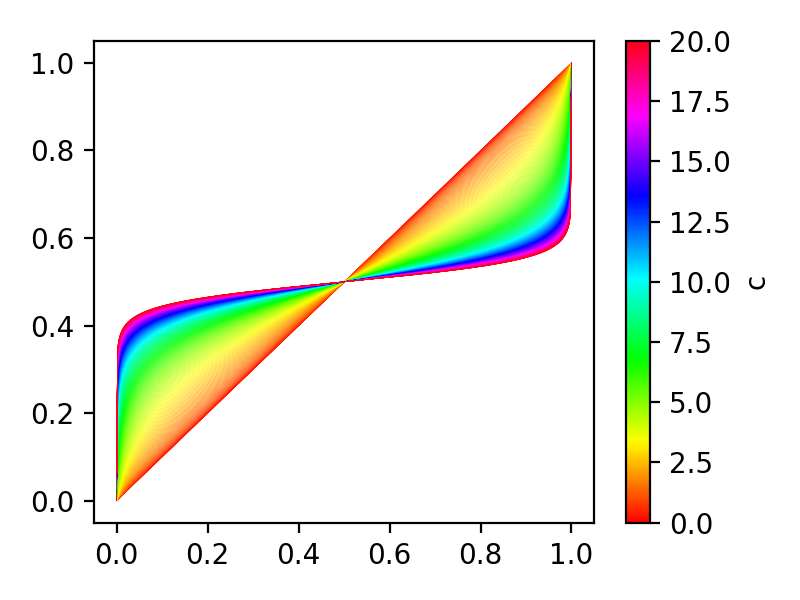
\includegraphics[width=\linewidth]{img/s_curve_c.png}
  \caption{$S^-1(x)$, sampled in $\left[S(-c), S(+c)\right]$ and normalized between 0 and 1}
  \label{fig:s_curve_c}
\end{figure}

To break the symmetry for the curve, to be able increase the conservation of the top rank while decreasing the conservation of the bottom ranked. The solution proposed is to take $r \cdot N$ samples for $\left[S(-c), S(0)\right]$ and $(1-r) \cdot N$ samples for $\left[S(0), S(c)\right]$. Figure~\ref{fig:s_curve_r} shows $\left[S(-4), S(4)\right]$ with $r \in \{0.25, 0.5, 0.75\}$.

\begin{figure}
  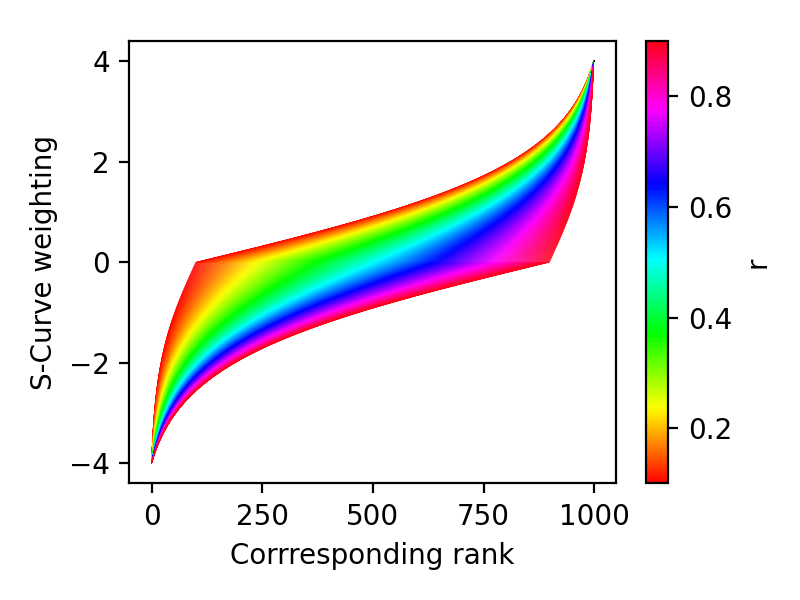
\includegraphics[width=\linewidth]{img/s_curve_r.png}
  \caption{Sampling $S^-1(x)$ with $r \cdot N$ samples for $\left[S(-c), S(0)\right]$ and $(1-r) \cdot N$ samples for $\left[S(0), S(c)\right]$}
  \label{fig:s_curve_r}
\end{figure}

\subsubsection{Evaluation}

\begin{table}[h]
  \caption{\textbf{S-curve}/Equal/Linear,  * : Binomial test p-value < 5\%}
  \centering
  \label{}
  \begin{tabular}{l c c c}
    \toprule
    Metric & St-Jean & Brunet & Oxquarry \\ \midrule
    AP     & \textbf{*84/0/0} & \textbf{*67/0/17} & \textbf{*77/0/7} \\
    RPrec  & \textbf{*74/6/4} & \textbf{*31/38/15} & \textbf{*58/13/13} \\
    HPrec  & \textbf{*66/3/15} & \textbf{*20/54/10} & \textbf{40/17/27} \\
    \bottomrule
  \end{tabular}
\end{table}

\begin{table}[h]
  \caption{\textbf{S-curve}/Equal/Single max,  * : Binomial test p-value < 5\%}
  \centering
  \label{}
  \begin{tabular}{l c c c}
    \toprule
    Metric & St-Jean  & Brunet & Oxquarry \\ \midrule
    AP     & \textbf{*55/0/29} & 37/0/47 & 9/0/75* \\
    RPrec  & \textbf{*61/2/21} & \textbf{*52/15/17} & 1/2/81* \\
    HPrec  & \textbf{47/1/36} & 0/0/84* & 14/1/69* \\
    \bottomrule
  \end{tabular}
\end{table}

\begin{table}[h]
  \caption{\textbf{Linear}/Equal/Single max,  * : Binomial test p-value < 5\%}
  \centering
  \label{}
  \begin{tabular}{l c c c}
    \toprule
    Metric& St-Jean  & Brunet & Oxquarry \\ \midrule
    AP    & \textbf{50/0/34} & 26/0/58* & 4/0/80* \\
    RPrec & \textbf{*52/2/30} & \textbf{*50/14/20} & 3/1/80* \\
    HPrec & \textbf{44/0/40} & 0/0/84* & 14/0/70* \\
    \bottomrule
  \end{tabular}
\end{table}

\begin{figure}
  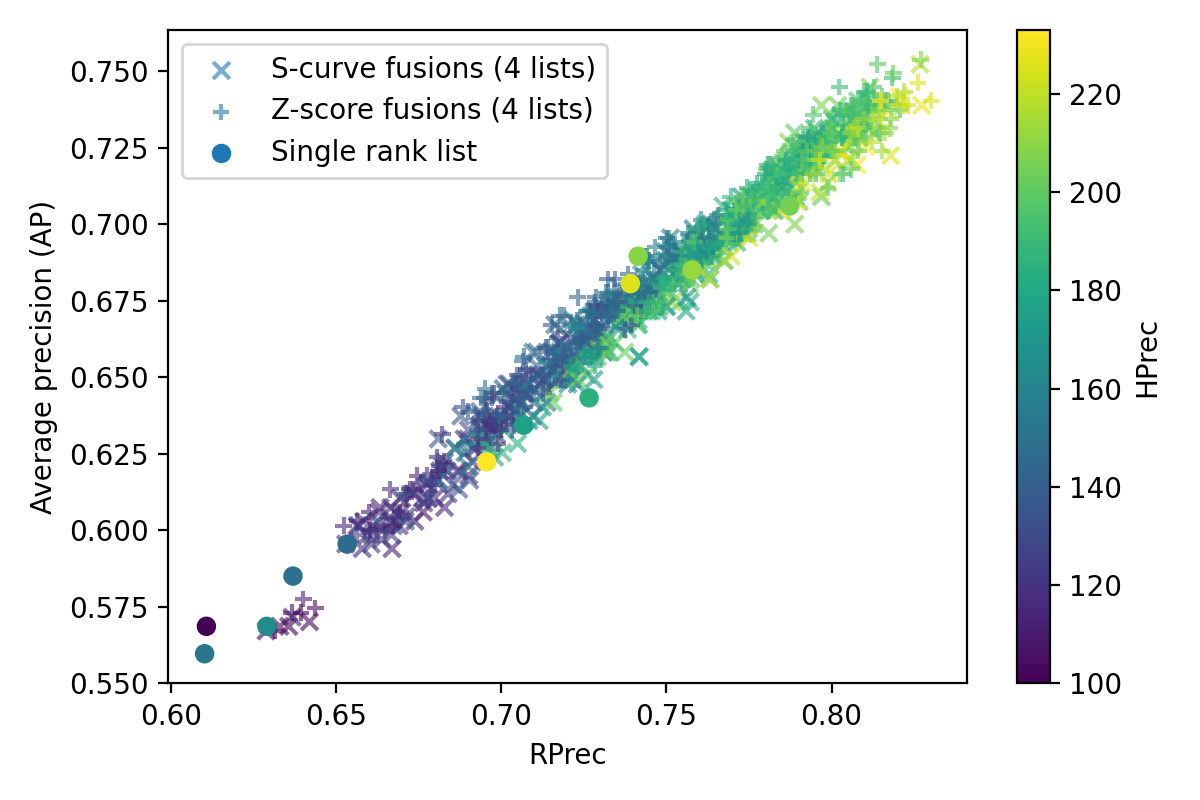
\includegraphics[width=\linewidth]{img/fusion_st_jean.png}
  \caption{}
  \label{fig:fusion_st_jean}
\end{figure}
\begin{figure}
  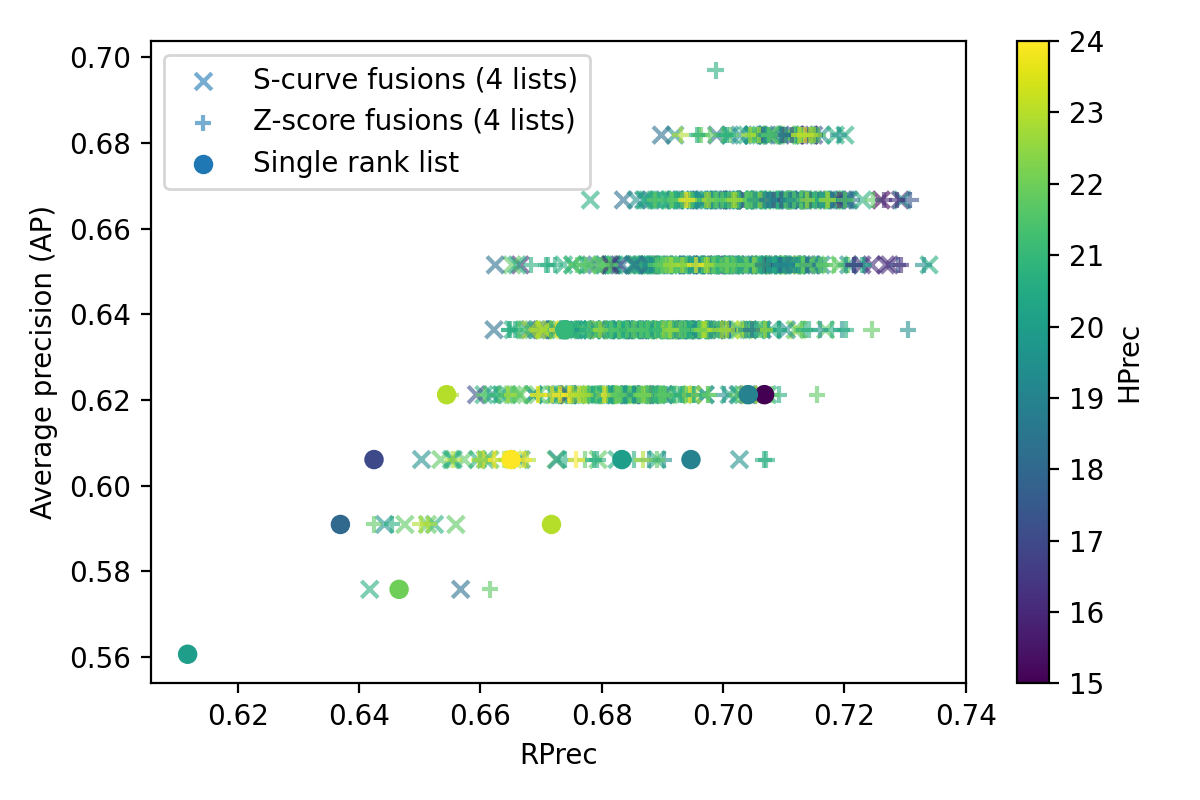
\includegraphics[width=\linewidth]{img/fusion_brunet.png}
  \caption{}
  \label{fig:fusion_brunet}
\end{figure}
\begin{figure}
  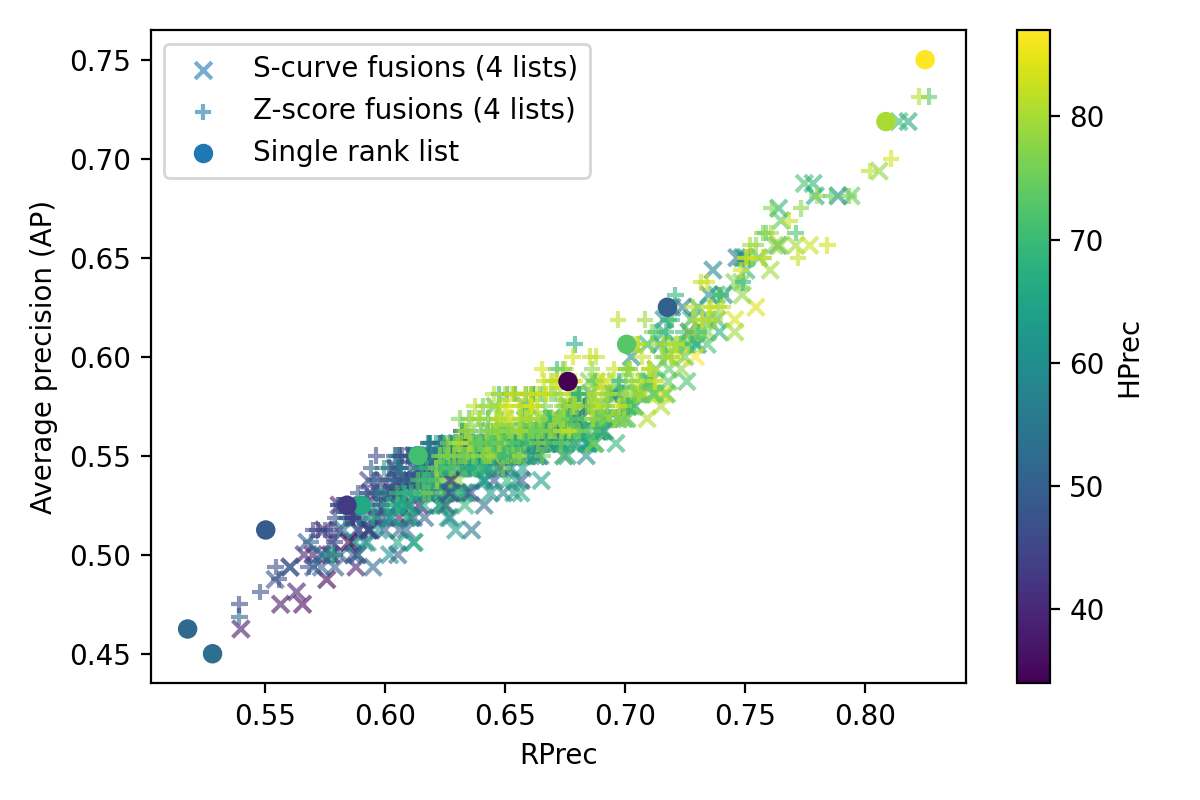
\includegraphics[width=\linewidth]{img/fusion_oxquarry.png}
  \caption{}
  \label{fig:fusion_oxquarry}
\end{figure}


\subsection{Authors Clustering}

To find clusters of authors, a possible way is to use a hierarchical clustering algorithm on a rank list.
In a rank list, each link indicate that both documents should belong to the same cluster in order of certainty.
The hardest task in this clustering scheme is to find the right cut in the rank list.
This cut should maximize the number of true links above the cut and the number of false links under the cut.
To find this cut, two apporaches were explored : one using a unsupervised clustering evaluation technique which is totaly unsupervised and another one using a linear model to learn to make this cut but it requires a training dataset.

\subsubsection{Agglomerative clustering}

The scikit-learn package~\cite{sklearn} provide an implementation bottom-up implementation of the hierarchical clustering, which is usually called agglomerative clustering.
Using this approach, at the start of the algorithm, each document belong to a different cluster.
Clusters are merge based on the scores in the rank list, each step the algorithm merge clusters using the minimal score based on the linkage criteria.
Multiple linkage criteria are available : \textit{ward} (metric that aim to minimize the variance of the cluster merged), \textit{average-linkage} (use the average score of each links of the cluster merged), \textit{complete-linkage} (use the maximal score of the cluster merged), \textit{single-linkage} (use the minimal score of the cluster merged).
Ward linkage was discarded since the implementation only allow euclidean distance for its computation.

\subsubsection{Learning the cut in a unsupervised way}

The silhouette score is a unsupervised clustering metric which evaluate a clustering result by mesureing the cohesion and separation of the clusters.
A large value indicate a good cohesion and good separation of the clusters.
Running the agglomerative clustering at each cut in the rank list then evaluating the clustering result using the silhouette score, the maximal shilhouette score position give a good indication where the best cut is.

\subsubsection{Learning the cut in a supervised way}



\subsection{Complexity}
